Wärme fließt grundsätzlich vom wärmeren Medium zum kälteren Medium - laut dem
zweiten Hauptsatz der Thermodynamik. Für die Umkehrung dieses Prozesses muss
Energie von außen zugeführt werden, z.B. durch eine Wärmepumpe, welche mechanische
Arbeit in das System steckt. Es gilt:
\begin{equation}
  Q_\su{1} = Q_\su{2} + A
\end{equation}
mit $Q_\su{1}$ als wärmere Wärmemenge, $Q_\su{2}$ als kältere Wärmemenge und $A$ als
aufzuwendende Arbeit.
\subsection{Merkmale der Wärmepumpe}
Eine Wärmepumpe besitzt im Wesentlichen drei entscheidende Faktoren: die Güteziffer,
den Massendurchsatz und den Wirkunsgrad.
\subsubsection{Güteziffer}
Die Güteziffer $\nu$ bezeichnet das Verhältnis zwischen der Arbeit $A$, welche aufzuwenden
ist, um die Wärme vom kälteren zum wärmeren Reservoir zu transportieren, und der
transportierten Wärmemenge $Q_\su{trans}$. Unter idealen Voraussetzungen gilt
\begin{equation}
      \nu_\su{ideal} = \frac{Q_\su{trans}}{A} = \frac{T_\su{1}}{T_\su{1}-T_\su{2}}.
\end{equation}
Hierfür muss die Wärmeübertragung jedoch reversibel sein. Für die Realität folgt
somit
\begin{equation}
  \nu_\su{real} < \frac{T_\su{1}}{T_\su{1}-T_\su{2}}.
\end{equation}
Je geringer die Temperaturunterschiede zwischen den Reservoiren sind, desto höher ist
die Güteziffer und desto weniger Arbeit muss die Pumpe verrichten.

Wird der Differenzenquotient durch die Differentialquotienten $\frac{dT_\su{1}}{dt}$
und $\frac{dQ_\su{1}}{dt}$ ersetzt, so folgt:
\begin{equation}
  \frac{dQ_\su{1}}{dt}= (m_\su{1}c_\su{w}+m_\su{k}c_\su{k})\frac{dT_\su{1}}{dt}
\end{equation}
$m_\su{1}c_\su{w}$ beschreibt die Wärmekapazität des Wassers im ersten Reservoir und
$m_\su{k}c_\su{k}$ die Wärmekapazität der Kupferschlange und des Eimers. Mit $N$
als gemittelte Leisungsaufnahme des Kompressors ergibt sich damit für die Güteziffer
$\nu$:
\begin{equation}
  \nu = (m_\su{1}c_\su{w}+m_\su{k}c_\su{k})\frac{dT_\su{1}}{dt} \cdot \frac{1}{N}
\end{equation}
\subsubsection{Massendurchsatz}
Der Massendurchsatz berechnet sich aus dem Quotienten $\frac{dT_\su{2}}{dt}$ als
\begin{equation}
  \frac{dQ_\su{2}}{dt}= (m_\su{2}c_\su{w}+m_\su{k}c_\su{k})\frac{dT_\su{2}}{dt}.
\end{equation}
Der Wärmeentzug geschieht durch die Verdampfung des Transportmediums. Dabei wird die
Verdampfungswärme $L$ pro Zeit- und Masseneinheit verbraucht. Aus diesem Zusammenhang folgt
\begin{align}
  \frac{dm}{dt} &= \frac{dQ_\su{2}}{dt} \cdot \frac{1}{L} \\
      &= (m_\su{2}c_\su{w}+m_\su{k}c_\su{k})\frac{dT_\su{2}}{dt} \cdot \frac{1}{L}.
\end{align}
\subsubsection{mechanische Kompressorleistung}
Wird ein Gasvolumen $V_\su{a}$ auf $V_\su{b}$ verkleinert, so leistet ein Kompressor
die Arbeit $A_\su{m}$ mit
\begin{equation}
  A_\su{m} = \int_{V_\su{a}}^{V_\su{b}}pdV
\end{equation}
Unter der Annahme, dass die Kompression adiabatisch erfolgt, gitl die Poissonsche
Gleichung:
\begin{equation}
  p_\su{a}V_\su{a}^\su{\kappa} = p_\su{b}V_\su{b}^\su{\kappa} = pV^\su{\kappa}
\end{equation}
$\kappa$ beschreibt das Verhältnis der Molwärme $c_\su{p}$ und $c_\su{v}$.
Für die mechanische Kompressorleistung $N_\su{mech}$ erigbt sich damit:
\begin{equation}
  N_\su{mech}= \frac{1}{\kappa-1}\Biggl(p_\su{b}\sqrt[\kappa]{\frac{p_\su{a}}{p_\su{b}}}-p_\su{a}
  \Biggr)\frac{\Delta V_\su{a}}{\Delta t} = \frac{1}{\kappa-1}\Biggl(p_\su{b}\sqrt[\kappa]{\frac{p_\su{a}}{p_\su{b}}}-p_\su{a}
  \Biggr)\frac{1}{\rho}\frac{\Delta m}{\Delta t}
\end{equation}
Die Dichte $\rho$ des Gases lässt sich über die ideale Gasgleichung bestimmen.
$p_\su{a}$ beschreibt den dazugehörigen Druck.
\subsection{Schematischer Aufbau der Wärmepumpe}
Eine Wärmepumpe ist typischerweise wie in Abbildung \ref{fig:1} aufgebaut.
\begin{figure}
\centering
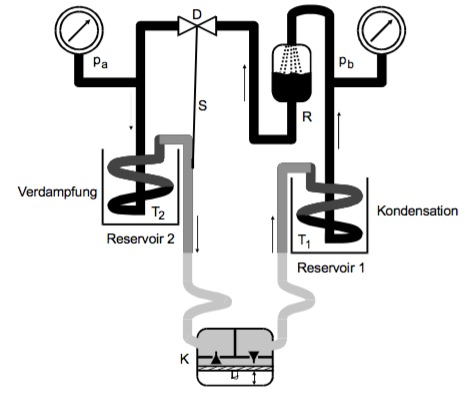
\includegraphics[width=10cm]{Bilder/schema.jpg}
\caption{schematischer Aufbau einer Wärmepumpe\,\cite{206}}
\label{fig:1}
\end{figure}
In der Wärmepumpe befindet sich ein reales Gas, welches durch Verdampfung Wärme aufnimmt
und sie bei Kondesation wieder abgibt. Dies wird als Phasenumwandlungsenergie bezeichnet
und es sollte idealerweise ein Gas mit hoher Kondensationswärme verwendet werden, damit
der Wirkungsgrad möglichst groß ist.

Das Gas bewegt sich im Kreislauf, welcher durch den Kompressor $K$ erzeugt wird. Dabei
durchströmt das Gas zwei Reservoire und das dazwischen liegende Drosselventil $D$.
An diesem Ventil entsteht ein Druckunterschied $p_\su{b}-p_\su{a}$. Dieses Ventil wird
über die Temperaturdifferenz gesteuert, da nur Gase in den Kompressor gelangen dürfen.

Im ersten Reservoir ist das Gas mit der Temperatur $T_\su{1}$ und dem Druck $p_\su{b}$
flüssig, im zweiten Reservoir ist das Gas mit der Temperatur $T_\su{2}$ und dem Druck
$p_\su{a}$ gasförmig. Das Wasser verdampft dann beim Durchströmen des Drosselventils
im zweiten Reservoir und entzieht diesem somit die Verdampfungswärme $L$. Das kalte, zweite
Reservoir, gibt somit Wärme ab.
Danach wird das Gas im Kompressor adiabatisch komprimiert, wodurch der Druck und die Temperatur
soweit ansteigen, bis sich das Gas im ersten Reservoir wieder verflüssigt. Hier wird die
Verdampfungswärme wieder abgegeben. Dadurch wird das erste Reservoir wieder aufgeheizt.
